\chapter{Algorithms}

In this section we will walk through some of the known matroid algorithms for solving some problems. Also we may derive some more information about the matroids themselves by looking at the solution of the given algorithms.

\section{Greedy algorithm}

The main algorithm is greedy one. One can already know the greedy algorithm for min spanning tree which is gradually putting lightest edges not forming cycle into the set. Now it will be pretty much the same only we will be maximizing and not minimizing. That is for minimizing we create a constant $C$ and subtract every value from it and still look for maximum which will indeed be a minimum with the original values.

First question is how to save all values for given matroid. Because the isze of $\I$ can be exponentially large. Therefore we will be working with so called \textbf{oracle}. That is for $X \subseteq E$ we ask if $X$ is independent $\in \I$ or not.

\begin{algorithm}[!ht]
	\caption{Greedy algorithm.}
	\begin{algorithmic}[1]
		\Require Matroid $\M = (E, \I)$ and weight function $w : E \to \R_0^+$.
		\Ensure $I \in \I$ with max $w(I) = \sum_{e \in I} w(e)$.
		\State Sort $E$ s.t. $w(e_1) \geq w(e_2) \geq \dots \geq w(e_n)$.
		\State $E_0 = \emptyset$
		\For{$i = 1, 2, \dots,n$}
			\If{$E_{i-1} + e_i \in \I$}
				\State $E_{i} = E_{i-1} + e_i$
			\Else
				\State $E_i = E_{i-1}$
			\EndIf
		\EndFor
		\State \Return $E_n$
	\end{algorithmic}
\end{algorithm}

\subsection{Correctness}

Firstly we can clearly see that $\forall i:  E_i \subseteq E$ and $E_i \in \I \Rightarrow E_n \in \I$ which also means that $E_n \in \I$ and $E_n \in \B$.

Now look at maximality. For contradiction $\exists E' \in \B$ s.t. $w(E') > w(E_n)$. See that $E_n$ is formed by $e_{i_1}, e_{i_2}, \dots, e_{i_r}$ if $r = \rank (\M)$ ($i_1 < i_2 < \dots < i_r$) and also $E'$ is formed by $e_{j_1}, e_{j_2}, \dots, e_{j_r}$ ($j_1 < j_2 < \dots < j_r$), where the lower index the higher weight. Therefore $\exists k$ s.t. $w(e_{i_k}) > w(e_{j_k})$ and lets take such smallest one. Now lets have $I_1 = \{e_{i_1}, \dots, e_{i_{k-1}}\}$ and $I_2 = \{e_{j_{1}}, \dots, e_{j_k}\}$ and apply (I3) because $|I_1| < |I_2|$ therefore $\exists l : I_1 + e_{j_l} \in \I$ and $w(e_{j_l}) \geq w(e_{j_k}) > w(e_{i_k})$ and $e_{j_l} \notin I_1$ which is a contradiction because algorithm would have chosen $e_{j_l}$ instead of $e_{i_k}$.

\subsection{Time complexity}

Firstly sorting $E$ is in $O(n \log n)$. Then the loop has $n$ repetitions where in every step we call an oracle. Lets say that the oracle has time complexity $t$ so the entire loop take $nt$ time. So altogether we obtain $O(n \log n + nt)$.

Lastly note that non-negative weight function is important for the algorithm to work. But we may see that this procedure can be used to define the matroid. Which we will talk about now.

\subsection{Defining matroid by greedy algorithm}

\begin{prop}
	We have $E$ finite non-empty set, let $\mathcal{F} \subseteq 2^E,\emptyset \in \mathcal{F}$ s.t. $\forall w : E \to \R_0^+$ greedy algorithm find max weighted member of $\mathcal{F}$, then $\mathcal{F}$ satisfies (I1),(I2) and (I3).
\end{prop}

\begin{proof}
	Firstly (I1) is easy, since $\emptyset \in \mathcal{F}$.
	
	Now take a look at (I2). By contradiction $I' \subseteq I$ and $I \in \mathcal{F}$ but $I' \notin \mathcal{F}$. WLOG $|I| = |I'| + 1$. We will define the weight function like this:
	
	$$
	w(e) = \left\{
	\begin{array}{l l}
		2 & \text{if } e \in I' \\
		1 & \text{if } e \in I \setminus I' \\
		0 & \text{otherwise}
	\end{array}
	\right..
	$$
	
	\noindent So $w(I) = 2 \cdot |I'| + 1$ and greedy algorithm find $|I'|$, but at least one element has to be skipped. So the weight of the result is $\leq 2(|I'| - 1) + 1 = 2 \cdot |I'| - 1 < w(I)$ which is a contradiction.
	
	Finally (I3) which is $I_1, I_2 \in \mathcal{F}, |I_1| < |I_2| : \exists e \in I_2 \setminus I_1 : I_1 + e \in \mathcal{F}$ and WLOG $|I_2| = |I_1| + 1$. By contradiction $I_1, I_2 \in \mathcal{F}, |I_1| = |I_2| - 1$ and $\forall e \in I_2 \setminus I_1 : I_! + e \notin \mathcal{F}$. Denote $k = |I_1|$. Lets define the weight function.
	
	$$
	w(e) = \left\{
	\begin{array}{l l}
		k+2 & \text{if } e \in I_1 \\
		k+1 & \text{if } e \in I_2 \setminus I_1 \\
		0 & \text{otherwise}
	\end{array}
	\right..
	$$
	
	\noindent Where $w(I_2) \geq |I_2| \cdot (k+1) = (k+1)^2$. The greedy algorithm firstly takes all $e \in I_1$ so after $k$ steps $E_k = I_1$, but then non-zero elements are skipped $(I_2 \setminus I_1)$ so the result has $w = I_1 \cdot (k+2) = k (k+2)$ but $k (k+2) = k^2 +2k < k^2 +2k + 1 = (k+1)^2$ so we got the contradiction.
\end{proof}

\section{Matroid intersection problem}

Firstly we must define this problem. As an \textbf{input} we have $\M_i = (E, \I_i)$ for $i = 1,2$ and \textbf{output} is to find max $I \in \I_1 \cap \I_2$. Firstly observe that there always exists a solution $\emptyset$.

\begin{thm}
	Having $\M_i = (E, \I_i)$ for $i = 1,2$ then
	
	$$
	\max_{I \in \I_1 \cap \I_2} |I| = \min_{E_1 \cup E_2 = E} \rank_1(E_1) + \rank_2(E_2).
	$$
	\label{min-max-thm}
\end{thm}

\begin{proof}
	For "$\leq$" we have $I \in \I_1 \cap \I_2, E_1 \cup E_2 = E$. We may consider it is disjoint since $E_2 = E \setminus E_1$ might only decrease the rank.
	
	$$
	\begin{array}{r c c c l}
		|I \cap E_1| & = & \rank_1 (I \cap E_1) & \leq & \rank_1(E_1) \\
		|I \cap E_2| & = & \rank_2 (I \cap E_2) & \leq & \rank_2(E_2) \quad \text{(sum both together)}\\
		|I| & & & \leq & \rank_1(E_1) + \rank_2(E_2) \\
	\end{array}
	$$
	
	Now "$\geq$" for which we will state the algorithm. Firstly start in $I = \emptyset$. Then $I \in \I_1 \cap \I_2$ construct $H$ bipartite graph with $I, X = E \setminus I$ parts. Create arc $y \to x$ if $(I - y) + x \in \I_1$ and arc $y \leftarrow x$ if $(I - y) + x \in \I_2$. Then define $X_1 = \{x \in X | I + x \in \I_1\}$ and $X_2 = \{x \in X | I + x \in \I_2\}$.
	
	\begin{enumerate}
		\item If $X_1 \cap X_2 = \emptyset$ we just add such element from intersection to $I$.
		\item Otherwise find $X_1 \to X_2$ path if there is one, and choose shortest one. That is $x_0 y_1 x_1 y_2 x_2 \dots y_k x_k$ this path where $x_0 \in X_1$ and $x_k \in X_2$. Now we update $I$ like this $I' = (I \setminus \{y_1, y_2, \dots, y_k\}) \cup \{x_0, x_1, x_2, \dots, x_k\}$. Clearly the size is bigger but it is independent? We will sketch the proof of this. We have to show that $I' \in \I_1 \cap \I_2$.
		
		For $I' \in \I_1$ we proceed by induction on $k$. Lets have $I \in \I$ and $(I - y_k) + x_k$ because $y_k \to x_k$ by the definition of arc it implies that it is $\in \I_1$. Lets denote $I_l = (I \setminus \{y_l, \dots, y_k\}) \cup \{x_l, \dots, x_k\} = (((I \setminus \{y_{l+1}, \dots, y_k\}) \cup \{x_{l+1}, \dots, x_k\}) - y_l) + x_l$ and $I_{l+1}$ is $\in \I_1$ by induction. So $I_l = (I_{l+1} - y_l) + x_l$, $I_l + x_l \in \I_1$ and $y_l \to x_l$ therefore $(I - y_l) + x_l \in \I_1$. We obtained two independent sets where $|I_l - x_l| = |(I - y_l) + x_l| - 1$ so by (I3) $\exists z \in (I - y_l) + x_l$ s.t. $(I_l - x_l) + z \in \I_1$.
		
		If $z = x_l$ we are done, otherwise if $z \neq x_l$ we set $(I - y_l + x_l) \setminus (I_l - x_l) = \{x_l, y_{l+1}, \dots, y_k\}$ so $\exists i : z = y_i$ $(I_l - x_l) + y_i \in \I_1$ and again apply (I3) so $\exists z' \in ((I_l - x_l) + y_i) \setminus (I - y_l)$ s.t. $(I - y_l) + z' \in \I_1$ and $z' = \{x_{l+1}, \dots, x_k\}$. This implies that $y_l \to z'$ which contradicts the shortest path. Hence we may remove $y_1, \dots, y_k$ and add $x_1, \dots, x_k$. Now we only need to show we may also add $x_0$. For showing $I' \in \I_2$ we would proceed similarly.
		
		\item Next step is what if the path does not exists? We want to show a partitioning $E_1$ and $E_2$ such that $X_2 \subseteq E_1$ and $X_1 \subseteq E_2$ and there is no edge from $E_2$ to $E_1$. We create the partition by adding all elements accesible from $X_1$ to $E_2$ and the rest will form $E_1$.

			\begin{observ}
				$\rank_i (E_i) = |I \cap E_i|, i =1,2$
			\end{observ}

			\begin{proof}[Proof of observation]
				For $i = 1$ we have that $\rank_1 (E_1) = |I \cap E_1|$ where $I \cap E_1$ is independent so $\rank_1(E_1) \geq \rank_1 (I \cap E_1))$. Assume that it is strict, i.e. $\rank_1 (E_1) > \rank_1 (I \cap E_1)$. Then $\exists x \in E_1 \setminus I : \rank(I \cap E_1 + x) > \rank(I \cap E_1)$ where $I \cap E_1 + x \in \I_1$. But $I + x \notin \I_1$ because this $x \in X_1$ and $E_1 \cap X_1 = \emptyset$. Also $(I - y) + x \in \I_1, y \in I \cap E_2$ from (I3) property. This all implies that there is an arc $y \to x$ which contradicts $E_1 \to E_2$ having no edge.
			\end{proof}

			With this observation we may see that $|I| = |I \cap E_1| + |I \cap E_2| = \rank_1 (E_1) + \rank_2(E_2)$ which finishes the proof of the theorem.
	\end{enumerate}
\end{proof}

\subsection{Time complexity}

We have at most $\rank (\rank \geq \rank_1 (E), \rank_2(E))$ iterations. Then also $2 \cdot |I| \cdot |X|$ queries for independent sets which is $\leq 2 \rank n$ and also we have $2 \cdot |X| \leq 2n$ other queries. Thus in total $O(\rank n)$ queries and if we denote the time for query as $\tau$ then the time complexity is $O(\tau \rank n)$. So all together it is $O(\rank^2 n \tau)$. Another remark is that it is known that we could obtain $O(\rank^{3/2} n \tau)$.

\subsection{Applications}

We will show us some usage of the theorem and the algorithm itself. The next theorems and algorithms are well known.

\subsubsection{Maximal matching in bipartite graph}

\begin{thm}
	$G$ is connected bipartite graph. Then maximum matching of $G$ has size equal to minimum vertex cover of $G$.
\end{thm}

\begin{proof}
	Let $G = (V_1 \cup V_2, E)$ and $\M_i = (E, \I_i)$ for $i = 1,2$. The matroids are defined by independ sets, where $E \supseteq I \in \I_i$ iff $\forall v \in V_i$ $\deg(v_i) \leq 1$ in $(V_1 \cup V_2, I)$. See an example on Fig. \ref{max-matching-matroid}. Therefore the maximal $I \in \I_1 \cap \I_2$ is equal to maximum matching of $G$. So by the theorem \ref{min-max-thm} $\exists E = E_1 \cup E_2$ s.t. $|I| = \rank_1 (E_1) + \rank_2 (E_2)$. Now take a look at the rank function. Denote $V_i' = \{v \in V_i | \exists e \in X : v \in e\}$ the rank function is $\rank_i (X) = |V_i'|$. Then from $\rank_1 (E_1)$ we get $|V_1'|$ and similary $|V_2'|$ and hence $V_1' \cup V_2'$. Therefore by the theorem $= |V_1'| + |V_2'| = |V_1' \cup V_2'|$ which is indeed a minimum vertex cover.

	\begin{figure}[!ht]\centering
		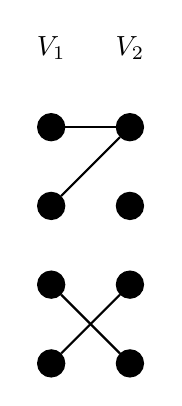
\begin{tikzpicture}[main/.style = {draw, circle, fill}, thick]
			\node (v1) {$V_1$};
			\node[right of = v1] (v2) {$V_2$};
			\node[main, below of = v1] (11) {};
			\node[main, below of = 11] (12) {};
			\node[main, below of = 12] (13) {};
			\node[main, below of = 13] (14) {};
			\node[main, below of = v2] (21) {};
			\node[main, below of = 21] (22) {};
			\node[main, below of = 22] (23) {};
			\node[main, below of = 23] (24) {};
			\draw (11) -- (21);
			\draw (12) -- (21);
			\draw (13) -- (24);
			\draw (14) -- (23);
		\end{tikzpicture}
		\caption{An example of matroids, where these edges are independent in $\M_1$ but not $\M_2$.}
		\label{max-matching-matroid}
	\end{figure}
\end{proof}

\subsubsection{Nash-Williams}

\begin{thm}[Nash-William]
	$G$ is connected (multi)graph, $k \in \N$ there exists $k$ pairwise disjoint spanning trees $\iff$ $\forall$ partition $V_1, \dots, V_k$ of $V$ we have $|\{e \in E, \forall i |e \cap V_i| \leq 1\}| \geq k (l-1)$.
\end{thm}

We will not prove this directly. Instead we will show more general matroid version which actually as a consequence proves this theorem.

\begin{thm}
	Let $\M = (E, \I)$ be a matroid and $k \in \N$. $\exists B_1, \dots, B_k$ disjoint bases of $\M$ $\iff$ $\forall S \in E$ $|E \setminus S| \geq k (\rank(E) - \rank(S))$.
\end{thm}

\begin{proof}
	Firstly we will create $k$ copies of $E$ that will be $E_0 = E \times \{1, \dots, k\}$. Now we will define two matroids. $\M_1 = (E_0, \I_1)$ where $X \in \I_1$ if $\forall i = 1, \dots, k \ X_i = \{e : (e,i) \in X\} \in \I$, that is from the original matroid $\M$. And also $\M_2 = (E_0, \I_2)$ where $X \in \I_2 \iff \forall e \in E$ there is at most one $i$ s.t. $(e,i) \in X$. Now we could say that it must be independent for every copy of $E$ and they have to be disjoint to be in the intersection.

	$\M$ has disjoint bases $B_1, \dots, B_k \iff \exists I \in \I_1 \cap \I_2$ s.t. $|I| \geq k \rank(E)$. And for the outline of the proof. Lets have $k$ disjoint bases $X = \{(e,i), \exists i : e \in B_i\}$ and for the other implication $|I| = k \rank(\M)$ constuct $B_i = \{e, (e,i) \in I\}$ and $|B_i| = \rank (B_i) \leq \rank(\M)$ since it is independent in $\M_2$ then $|I| = |\bigcup_i B_i|$ so $|B_i| = \rank(\M)$ for $i = 1,2, \dots, k$.

	"$\Rightarrow$" Now $B_1, \dots, B_k$ be disjoint bases of $\M$. See the following computation.

	$$
	\begin{aligned}
		|E \setminus S| &\geq \sum_{i=1}^k |B_i \cap (E \setminus S)| = \sum_{i=1}^k |B_i \setminus (B_i \cap S)| = \sum_{i=1}^k |B_i| - |B_1 \cap S| \\
		&= \sum_{i=1}^k \rank(\M) - |B_i \cap S| = \sum_{i=1}^k \rank(\M) - \rank(B_i \cap S) \geq \sum_{i=1}^k \rank(\M) - \rank(S) = k \cdot (\rank(\M) - \rank(S))
	\end{aligned}
	$$

	"$\Leftarrow$" Assume $\forall S \subseteq E : |E \setminus S| \geq k \cdot (\rank(E) - \rank(S))$. Now $|I| = \rank_1 (E_1) + \rank_2 (E_2)$ by the theorem \ref{min-max-thm}. If $(e,i) \in E_2$ we can add all $(e,j)$ to $E_2$ and $\rank_2(E_2)$ does not increases. Let $E_2 = E' \times \{1, \dots, k\}$ and $E_1 = E' \setminus E_2$. Set $S = E \setminus E'$. Then we have the following

	$$
	\begin{aligned}
		\rank_1 (E_1) &= \sum_{i=1}^k \rank(E_{1,i}) = k \cdot \rank(S) \\
		\rank_2 (E_2) &= |E'|\\
		\rank_1(E_1) + \rank_2(E_2) &= k \cdot \rank(S) + |E'| = k \cdot \rank(S) + |E \setminus S| \geq k \cdot \rank(S) + k \cdot \rank(E) - k \cdot \rank(S) = k \cdot \rank(\M)
	\end{aligned}
	$$

	\noindent So it can be decomposed to $B_1, \dots, B_k$ disjoint bases.
\end{proof}
